\def\year{2022}\relax
%File: formatting-instructions-latex-2022.tex
%release 2022.1
\documentclass[letterpaper]{article} % DO NOT CHANGE THIS
\usepackage{aaai22}  % DO NOT CHANGE THIS
\usepackage{times}  % DO NOT CHANGE THIS
\usepackage{helvet}  % DO NOT CHANGE THIS
\usepackage{courier}  % DO NOT CHANGE THIS
\usepackage[hyphens]{url}  % DO NOT CHANGE THIS
\usepackage{graphicx} % DO NOT CHANGE THIS
\urlstyle{rm} % DO NOT CHANGE THIS
\def\UrlFont{\rm}  % DO NOT CHANGE THIS
\usepackage{natbib}  % DO NOT CHANGE THIS AND DO NOT ADD ANY OPTIONS TO IT
\usepackage{caption} % DO NOT CHANGE THIS AND DO NOT ADD ANY OPTIONS TO IT
\DeclareCaptionStyle{ruled}{labelfont=normalfont,labelsep=colon,strut=off} % DO NOT CHANGE THIS
\frenchspacing  % DO NOT CHANGE THIS
\setlength{\pdfpagewidth}{8.5in}  % DO NOT CHANGE THIS
\setlength{\pdfpageheight}{11in}  % DO NOT CHANGE THIS
%
% These are recommended to typeset algorithms but not required. See the subsubsection on algorithms. Remove them if you don't have algorithms in your paper.
\usepackage{algorithm}
\usepackage{algorithmic}

\usepackage{graphicx, caption, subcaption}
\usepackage{amsmath}
\usepackage{color}
\usepackage{multirow}
\usepackage{booktabs}
\usepackage{bbm}
\usepackage{enumitem}
\usepackage[flushleft]{threeparttable}
\usepackage{makecell}
% \usepackage{hyperref}
\usepackage{amsfonts}
\usepackage[normalem]{ulem}
\newcommand{\KZ}[1]{\textcolor{blue}{Kenny: #1}}
\newcommand{\cut}[1]{}
%
% These are are recommended to typeset listings but not required. See the subsubsection on listing. Remove this block if you don't have listings in your paper.
\usepackage{newfloat}
\usepackage{listings}
\lstset{%
	basicstyle={\footnotesize\ttfamily},% footnotesize acceptable for monospace
	numbers=left,numberstyle=\footnotesize,xleftmargin=2em,% show line numbers, remove this entire line if you don't want the numbers.
	aboveskip=0pt,belowskip=0pt,%
	showstringspaces=false,tabsize=2,breaklines=true}
\floatstyle{ruled}
\newfloat{listing}{tb}{lst}{}
\floatname{listing}{Listing}
%
%\nocopyright
%
% PDF Info Is REQUIRED.
% For /Title, write your title in Mixed Case.
% Don't use accents or commands. Retain the parentheses.
% For /Author, add all authors within the parentheses,
% separated by commas. No accents, special characters
% or commands are allowed.
% Keep the /TemplateVersion tag as is
\pdfinfo{
/Title (Product Categorization for Multiple Evolving Businesses)
/Author (AAAI Press Staff, Pater Patel Schneider, Sunil Issar, J. Scott Penberthy, George Ferguson, Hans Guesgen, Francisco Cruz, Marc Pujol-Gonzalez)
/TemplateVersion (2022.1)
}

% DISALLOWED PACKAGES
% \usepackage{authblk} -- This package is specifically forbidden
% \usepackage{balance} -- This package is specifically forbidden
% \usepackage{color (if used in text)
% \usepackage{CJK} -- This package is specifically forbidden
% \usepackage{float} -- This package is specifically forbidden
% \usepackage{flushend} -- This package is specifically forbidden
% \usepackage{fontenc} -- This package is specifically forbidden
% \usepackage{fullpage} -- This package is specifically forbidden
% \usepackage{geometry} -- This package is specifically forbidden
% \usepackage{grffile} -- This package is specifically forbidden
% \usepackage{hyperref} -- This package is specifically forbidden
% \usepackage{navigator} -- This package is specifically forbidden
% (or any other package that embeds links such as navigator or hyperref)
% \indentfirst} -- This package is specifically forbidden
% \layout} -- This package is specifically forbidden
% \multicol} -- This package is specifically forbidden
% \nameref} -- This package is specifically forbidden
% \usepackage{savetrees} -- This package is specifically forbidden
% \usepackage{setspace} -- This package is specifically forbidden
% \usepackage{stfloats} -- This package is specifically forbidden
% \usepackage{tabu} -- This package is specifically forbidden
% \usepackage{titlesec} -- This package is specifically forbidden
% \usepackage{tocbibind} -- This package is specifically forbidden
% \usepackage{ulem} -- This package is specifically forbidden
% \usepackage{wrapfig} -- This package is specifically forbidden
% DISALLOWED COMMANDS
% \nocopyright -- Your paper will not be published if you use this command
% \addtolength -- This command may not be used
% \balance -- This command may not be used
% \baselinestretch -- Your paper will not be published if you use this command
% \clearpage -- No page breaks of any kind may be used for the final version of your paper
% \columnsep -- This command may not be used
% \newpage -- No page breaks of any kind may be used for the final version of your paper
% \pagebreak -- No page breaks of any kind may be used for the final version of your paperr
% \pagestyle -- This command may not be used
% \tiny -- This is not an acceptable font size.
% \vspace{- -- No negative value may be used in proximity of a caption, figure, table, section, subsection, subsubsection, or reference
% \vskip{- -- No negative value may be used to alter spacing above or below a caption, figure, table, section, subsection, subsubsection, or reference

\setcounter{secnumdepth}{2} %May be changed to 1 or 2 if section numbers are desired.

% The file aaai22.sty is the style file for AAAI Press
% proceedings, working notes, and technical reports.
%

% Title

% Your title must be in mixed case, not sentence case.
% That means all verbs (including short verbs like be, is, using,and go),
% nouns, adverbs, adjectives should be capitalized, including both words in hyphenated terms, while
% articles, conjunctions, and prepositions are lower case unless they
% directly follow a colon or long dash
\title{Enhanced Semantic Space: Integrate Concepts \\to Unify Dynamic Multi-Domain Product Categorization}
\author{
    %Authors
    % All authors must be in the same font size and format.
    % Written by AAAI Press Staff\textsuperscript{\rm 1}\thanks{With help from the AAAI Publications Committee.}\\
    Submission ID: 8044
    % AAAI Style Contributions by Pater Patel Schneider,
    % Sunil Issar,\\
    % J. Scott Penberthy,
    % George Ferguson,
    % Hans Guesgen,
    % Francisco Cruz\equalcontrib,
    % Marc Pujol-Gonzalez\equalcontrib
}
% \affiliations{
%     %Afiliations
%     \textsuperscript{\rm 1}Association for the Advancement of Artificial Intelligence\\
%     % If you have multiple authors and multiple affiliations
%     % use superscripts in text and roman font to identify them.
%     % For example,

%     % Sunil Issar, \textsuperscript{\rm 2}
%     % J. Scott Penberthy, \textsuperscript{\rm 3}
%     % George Ferguson,\textsuperscript{\rm 4}
%     % Hans Guesgen, \textsuperscript{\rm 5}.
%     % Note that the comma should be placed BEFORE the superscript for optimum readability

%     2275 East Bayshore Road, Suite 160\\
%     Palo Alto, California 94303\\
%     % email address must be in roman text type, not monospace or sans serif
%     publications22@aaai.org
% %
% % See more examples next
% }

% %Example, Single Author, ->> remove \iffalse,\fi and place them surrounding AAAI title to use it
% \iffalse
% \title{My Publication Title --- Single Author}
% \author {
%     Author Name
% }
% \affiliations{
%     Affiliation\\
%     Affiliation Line 2\\
%     name@example.com
% }
% \fi

% \iffalse
% %Example, Multiple Authors, ->> remove \iffalse,\fi and place them surrounding AAAI title to use it
% \title{My Publication Title --- Multiple Authors}
% \author {
%     % Authors
%     First Author Name,\textsuperscript{\rm 1}
%     Second Author Name, \textsuperscript{\rm 2}
%     Third Author Name \textsuperscript{\rm 1}
% }
% \affiliations {
%     % Affiliations
%     \textsuperscript{\rm 1} Affiliation 1\\
%     \textsuperscript{\rm 2} Affiliation 2\\
%     firstAuthor@affiliation1.com, secondAuthor@affilation2.com, thirdAuthor@affiliation1.com
% }
% \fi


% REMOVE THIS: bibentry
% This is only needed to show inline citations in the guidelines document. You should not need it and can safely delete it.
\usepackage{bibentry}
% END REMOVE bibentry

\newcommand{\TODO}[1]{\textcolor{red}{(todo: #1)}}
\newcommand{\secref}[1]{Section \ref{#1}}
\newcommand{\figref}[1]{Figure \ref{#1}}
\newcommand{\eqnref}[1]{Eq. (\ref{#1})}
\newcommand{\tabref}[1]{Table \ref{#1}}
\newcommand{\exref}[1]{Example \ref{#1}}
\newcommand{\tabincell}[2]{\begin{tabular}{@{}#1@{}}#2\end{tabular}}

\begin{document}

\maketitle

\begin{abstract}
    Product categorization is to assign a product with a suitable category, which is usually organized in a predefined taxonomy.
    As e-commerce platforms developing different business lines, a special but challenging categorization scenario emerges, where there are multiple domain-specific category taxonomies and each of them evolves dynamically over time. 
    In order to unify the categorization process and jointly utilize the cross-domain data, we propose a two-stage taxonomy-agnostic framework that relies solely on calculating the semantic relatedness 
    between product titles and category names in the vector space. 
    However, pure vector matching may fall for the surface form of text, 
    % \textbf{indulges the surface form of the text dominating the score model}, 
    and we thus further leverage the universal ``knowledge'' across different business domains to complement textual semantics.
    % to mitigate this issue. 
    We design a heuristic retrieval strategy and pretrain a contrastive ranking model with the help of ``concept'', which resembles the shared keyword knowledge cross domains. 
    % In the end, the semantic matching is the backbone of our framework, but the concept knowledge is the fuel to power the unified model. 
    Our comprehensive experiments show that our method outperforms existing sophisticated approaches quantitatively and efficiently on dynamical multi-domain taxonomies. 
\end{abstract}

\section{Introduction}

Protein$-$protein interactions (PPIs) are of central importance for the majority of biological functions, such as signal transduction, metabolic pathways, molecular dynamics, and protein networks\cite{Hoffmann.Krallinger.ea:2005}, for they serve as the most fundamental building blocks of the entire interacademic systems of any organisms. Collecting data on pairwise interaction relationships is essential for multiple purpose, including identification of modules with certain functionality\cite{Spirin.Mirny.03}, mapping diseases to dominated genes\cite{Ideker.Sharan.08}, and after all, understanding wholistic metabolic/genetic networks from a system biology perspective.

A lot of databases have been built to store protein and genetic interactions from major model organism species and are available in various standardized formats, such as MINT\cite{Zanzoni.Montecchi-Palazzi.ea:2002}, BIND\cite{Bader.ea:2003}, BIOGRID\cite{DBLP:journals/nar/StarkBRBBT06}, etc. Among those mainstream databases, the data largely rely on voluntary reports by scientists or researchers, besides, comprehensive curation efforts become indispensable for the sake of accuracy. However, the amount of biology-related literatures with respect to protein interactions grows explosively and thus make it either impossible or impractical to manually detect PPI information anymore.

Considering huge amount of PPI information with great wealth hidden in published papers, in recent years, numerous mining techniques have been proposed that aim to extract PPI information automatically from free text, especially machine learning, information retrieval, and natural language processing\cite{DBLP:journals/bib/WinnenburgWPDS08}.These approaches can be roughly categorized into three classes: co$-$occurrence, rule$-$based, and machine learning. 

Co$-$occurrence is the approach with most simplicity and naivete. Just as its name implies, this method intends to find out pairs of proteins that co-occur in the same context. The scope of "same context" ranges from phrase, sentence, paragraph to whole abstract, even document. The underlying assumption is that whenever two proteins are mentioned together by authors, chances are high that there is some kind of relationship between them. However, however, in-context closeness even semantic relation does not necessarily represent actual biological interaction. As a consequence, a large fraction of candidate pairs are mismatched inevitably, causing a high recall but low precision.

The second approach is rule-based extraction, in other words, pattern matching. There are many types of rules, most of them concern natural language processing (NLP). One way is to specify hand-crafted regular expressions before hand, which mostly lean on language usage preference. Besides, by using full or partial (shallow) parsing strategies, more information would be acquired, such as part-of-speech taggers, local dependencies between syntactic components, context-free grammar\cite{DBLP:journals/bioinformatics/TemkinG03}, and full sentence structure. Compared to co$-$occurrence, rule-based approach enjoy better precision but much lower recall. In addition, since the rules are usually derived from training data, that is to say, the improper choice of training data would be significantly lethal, therefore quality of extraction is invariably instable and may not applicable to other data.

The third and most commonly used approach use machine learning techniques, in this case, the task to extract protein$-$protein interactions turns out to be a binary classification problem. Each protein pairs are represented along with a set of features, which is associated with their context, then a well$-$defined classifier gives the answer whether the candidate protein pairs is classified to be qualified PPI. (TO BE FURTHER FILLED!!!)

In this paper, we introduce a general bootstrapping framework for Protein$-$protein interaction extraction from natural text.Our method differs from most of the previous works in three aspects:

(1)The extraction process is driven by only tiny fraction of training data, which are regarded as seed data. In each round, it would derive reliable patterns automatically from seed data, then extract more positive PPI pairs consequently, what's more, the seed data would be augmented by the newly extracted results with high confidence.

(2)multiple graph kernel. 

(3)various evaluation.




\section{Task Definition}
We formulate our recommendation problem as the sequential recommendation or next item prediction. Assume that each user $u$ has a corresponding interaction sequence $S_u$, which can be represented as \[S_u=\{(x_1,c_1,T_1),(x_2,c_2,T_2),...,(x_T,c_T,T_T)\},\] where $x_j$ denotes the $j$-th news articles that user $u$ interacts with, and $c_j$ denotes the context embedding vectors of the corresponding articles, and $T_j$ denotes the intra-session temporal information of the corresponding interactions. Noted that each user $u$ only appear once, $S_u$ is corresponding to different sessions. Each $S_u$ starts at time $T_u$.

The intra-session temporal information $T_j$ contains two part. One is the time of $j$-th interaction $Tc_j$, which means the time user $u$ \textit{clicks} the $j$-th article and reflects it's position in $S_u$. The other is the \textit{publish} time of $j$-th article $Tp_j$, reflecting the refreshness of it. The $T_u$ reflects the inter-session temporal information because sessions with close start time are more related to each other.

Given a target user $u$ with her sequential of interactive behaviors over items $S_u$, our personalized next-item recommendation task is to predict $x_{T+1}$ that the target user $u$ is most likely to access in his/her next visit. Noted that the long term history of user $u$ is invisible, and we're supposed to predict $x_{T+1}$ in real-time right away after sequential of interactive behaviors from $x_1$ to $x_T$. The whole procedure is depicted in \figref{fig:representation}.
\section{Approach}
%We first present our methods for testing short circuits in
%models, then modify some of these methods to create
%training data to reverse the short circuit problem
%and enhance the robustness of the models.
% 
%\subsection{Proxy Test for Short Circuit}
%We propose two types of approaches that can be used as proxy test for short circuits.
%One is through inspecting attention maps in
%the models under a white-box setting.
%The other is to generate new test cases by applying different operations on correct choices under a black-box setting.
%
%
%\subsubsection*{White-box Attention Weights~(AW)}
%One intuitive way to detect if an attention-based model is 
%exploiting short circuits is to visualize its attention map. 
%Given a well-trained model and a correctly answered MCQ  in the 
%form of \textit{[CLS] premise [SEP] choice [SEP]}, 
%where \textit{[CLS]} and \textit{[SEP]} are model-dependent 
%delimiters and \textit{choice} refers to the correct choice, 
%we first tokenize the input, feed the token sequence into the model, 
%and extract the attention map of all attention heads from the 
%last encoder layer.
%
%The attention maps are visualized through off-the-shelf tool~\cite{vig-2019-multiscale}
%into user-friendly demo as shown in \figref{fig:att-goodex}. 
%Human annotators are then asked to determine whether there exists 
%strong attention connections from the correct choice to the premise. 
%We consider the MCQ is solved without short-circuiting only if 
%over half of the annotators label it as having strong attention 
%connections. 
%
%Though accurate, such manual annotation is cost-prohibitive to be 
%scaled to larger tests. To remedy this issue, we propose 
%a rule-based procedure to automatically detect the short circuit 
%behavior of a model on MCQ. Specifically, we aggregate the 
%attention maps into one individual map by max-pooling over all 
%attention heads. Then we check if there exists at least one 
%attention score between token in the choice and token in the premise 
%higher than threshold $t_1$ or at least two higher than threshold 
%$t_2$, excluding special tokens like comma and period. 
%We consider that the model not short-circuiting on this MCQ if 
%neither of the two conditions is met. In practice, the 
%threshold $t_1$ and $t_2$ are tuned so as to maximally simulate 
%human annotation. The pseudo-code is shown in Algorithm \ref{AW}.
%
In this section, we first present our methods for testing short circuits in models, and then modify some of these methods to create training data to address the short circuit problem and enhance model robustness.

\subsection{Proxy Test for Short Circuit}
Since no existing method can definitively prove if a model is short-circuiting on a question, we propose two types of approaches that serve as proxy tests for short circuits. These approaches reveal the effects of model short-circuiting, though they can't directly prove the short-circuit itself, similar to dark matter. One approach involves inspecting attention maps in models under a white-box setting, while the other generates new test cases by applying different operations on correct choices under a black-box setting.

\subsubsection*{White-box Attention Weights~(AW)}

One intuitive way to detect if an attention-based model is exploiting short circuits is to visualize its attention map. Given a well-trained model and a correctly answered MCQ in the form of \textit{[CLS] premise [SEP] choice [SEP]}, where \textit{[CLS]} and \textit{[SEP]} are model-dependent delimiters and \textit{choice} refers to the correct choice, we first tokenize the input, feed the token sequence into the model, and extract the attention map of all attention heads from the last encoder layer.

The attention maps are visualized through an off-the-shelf tool~\cite{vig-2019-multiscale} into a user-friendly demo, as shown in \figref{fig:att-goodex}. Human annotators are then asked to determine whether there exists strong attention connections from the correct choice to the premise. We consider the MCQ to be solved without short-circuiting only if over half of the annotators label it as having strong attention connections.

Although accurate, such manual annotation is cost-prohibitive to be scaled to larger tests. To remedy this issue, we propose a rule-based procedure to automatically detect the short circuit behavior of a model on MCQ. Specifically, we aggregate the attention maps into one individual map by max-pooling over all attention heads. Then we check if there exists at least one attention score between a token in the choice and a token in the premise higher than threshold $t_1$, or at least two higher than threshold $t_2$, excluding special tokens like comma and period. We consider the model to not be short-circuiting on this MCQ if neither of the two conditions is met. In practice, the thresholds $t_1$ and $t_2$ are tuned to maximally simulate human annotation. The pseudo-code is shown in Algorithm \ref{AW}.


\begin{algorithm}
\small
	\caption{Attention Weight Thresholding}
	\label{AW}
\hspace*{0.02in} {\bf Input:} 
premise $P$, correct choice $C$, model $M$,  threshold $t_1$ and $t_2$. \\
\hspace*{0.02in} {\bf Output:}
binary 0/1 label $L$.
	\begin{algorithmic}[1]
		\State initialize counters $c_1$ and $c_2$ to 0.
		\State tokenize the formatted input as sequence of tokens $S$.
		\State feed $S$ into $M$ and extract the last layer's attention maps $Attn_{all}$.
		\State aggregate $Attn_{all}$ into $Attn_{max}$ by max-pooling over all attention heads.
		\For{$w_1$ in $C$}
		\For{$w_2$ in $P$}
		\If{$Attn_{max}(w_1, w_2)> t_1$}
				$c_1$ += 1
		\EndIf
		\If{$Attn_{max}(w_1, w_2) > t_2$}
				$c_2$ += 1
		\EndIf
		\EndFor
		\EndFor
		\State output 1 if $c_1>0$ or $c_2\geq 2$ and 0 otherwise.
	\end{algorithmic}
\end{algorithm}

\subsubsection*{Black-box Choice Operator}
\label{sec:proxy}
While attention-based testing methods can detect short circuits within the encoder directly, they don't directly detect short circuits in the end-to-end MCQ model, which also includes a linear layer above the attention-based pretrained language model. Additionally, these methods are limited to a family of models with inherent attention mechanisms.

A more desirable approach is an automatic end-to-end black-box test that is model-independent. In black-box testing, if a model correctly answers an MCQ, we slightly modify the MCQ by applying a certain``operation'' on the original correct choice to produce another wrong choice. The newly generated MCQ must share the same correct choice as the original question. By observing the model's response to the second MCQ, we can infer whether the model short-circuits on the original MCQ.If the model still selects the correct choice, then we consider it to have passed the test and not short-circuited on the original MCQ. The challenge now is how to construct the new wrong choice by implementing the operation in various ways.

In this paper, we consider the operations listed in \tabref{table:proxyop}. Some of the operations were mentioned in previous literature, while others are proposed here (marked with *).
The first line in each cell describes the operation, and the next two lines provide an example of constructing a false choice from a choice in the original question. An operation may either preserve (p) the truth value (\crosssymbol $\rightarrow$ \crosssymbol) or change (c) the truth value of the choice (\checksymbol $\rightarrow$ \crosssymbol).

\begin{table}[th]
        \centering
        \scriptsize
        \begin{tabular}{l|l}
                \toprule
                \textbf{Oper.} &\textbf{Description and Example}\\
                \hline
                \multirow{3}{*}{Neg+} & Add negation (c) \\
                & \textit{They called the police to come to my house. \checksymbol} \\
                & \textit{They {\color{olive}{didn't}}  called the police to come to my house. \crosssymbol} \\
                \hline
                \multirow{3}{*}{Neg-} &Remove negation (c) \\
                & \textit{Ben {\color{olive} never} starts working out. \checksymbol} \\
                & \textit{Ben starts working out. \crosssymbol}\\
                \hline

                \multirow{3}{*}{NER} &Randomly replace person names (c)\\
                 & \textit{A big wave knocked {\color{olive} Mary} down . \checksymbol} \\
                & \textit{A big wave knocked {\color{olive} Kia} down . \crosssymbol} \\
                \hline
                \multirow{3}{*}{PR*} & Switch pronoun by gender or quantity (c)\\
        &\textit{{\color{olive} She} had a great time .\checksymbol} \\
        &\textit{{\color{olive} He} had a great time . \crosssymbol} \\
                \hline
                \multirow{3}{*}{PI*} &Instantiate pronoun by randome person (c) \\
        &\textit{{\color{olive} They} gave Tom a new latte with less ice . \checksymbol}\\
        &\textit{{\color{olive} Nathanael} gave Tom a new latte with less ice . \crosssymbol}\\
                \bottomrule
%               \hline
                \multirow{3}{*}{Adv} &Add adverbs for emphasis (c) \\
                &\textit{The ocean was a calm as a bathtub .\crosssymbol} \\
                &\textit{{\color{olive} In fact} the ocean was a calm as a bathtub .\crosssymbol} \\
                \hline
               \multirow{3}{*}{CO*} & Crossover: Swap the true choices between two questions (p)\\ 
	&\textit{\color{olive}Josh got sick . \checksymbol} \\
	&\textit{\color{olive}{She had a great time .\crosssymbol}}  \\
\hline
                \multirow{3}{*}{Syn} &Replace adj/adv with synonym (p) \\
                &\textit{Dawn felt {\color{olive} happy} about getting away with it . \crosssymbol} \\
                &\textit{Dawn felt {\color{olive} glad} about getting away with it . \crosssymbol} \\

		\bottomrule
               \multirow{3}{*}{MT*} & Mutate: Swap two consecutive words (c) \\
		& \textit{Deb said yes {\color{olive} to} {\color{olive} Tim} 's marriage proposal. \crosssymbol} \\
		& \textit{Deb said yes {\color{olive} Tim} {\color{olive} to} 's marriage proposal .\crosssymbol} \\
               \hline
\multirow{3}{*}{Voice} &Swap subject and object (c) \\
        & \textit{{\color{olive}{Kara}} asked {\color{olive}{the neighbors}}  not to litter in their yard . \checksymbol} \\
        &\textit{{\color{olive}{the neighbors}} asked  {\color{olive}{Kara}}  not to litter in their yard . \crosssymbol}\\
                \bottomrule
        \end{tabular}
        \caption{A number of operations considered for proxy testing. 
First line in each cell describes the operation, the next two lines
give an example of how to construct a false choice from a choice of
the original question. An operation may either 
preserve (p) the truth value (\checksymbol $\rightarrow$ \checksymbol, \crosssymbol $\rightarrow$ \crosssymbol) or change (c) the truth value of
the choice (\checksymbol $\rightarrow$ \crosssymbol).  }
        \label{table:proxyop}
\end{table}

Inspired by boundary testing in software engineering, we can classify these operations into three equivalent classes (three vertical sections in \tabref{table:proxyop}), depending on the nature of the \textit{false} choice constructed:
\begin{enumerate}
\item The syntax and semantics are correct, and the \textit{false} choice appears similar to the \textit{true} choice.
\item The syntax and semantics are correct, and the \textit{false} choice appears distinct from the \textit{true} choice.
\item Either syntax or semantics is incorrect.
\end{enumerate}

The last class is not suitable for testing short circuits because the model may answer the proxy question correctly by eliminating the false choice due to errors in it, not by considering the premise.

We focus on perturbations on negation~\cite{checklist2020acl}, NER~\cite{checklist2020acl}, and pronouns in the first class and adverbial~\cite{wsp2020acl}, crossover, and synonym~\cite{checklist2020acl,wsp2020acl} in the second class.

While most of the operations are self-explanatory, the \textit{crossover} operation is unique and deserves special attention. Inspired by molecular biology, for each MCQ in the dataset that the model answers correctly, we substitute the original false choice with the true choice from another randomly sampled MCQ. The substituted choice remains false in the proxy question. The operation can be visually explained in \figref{fig:cross}.

\begin{figure}[th]
\centering
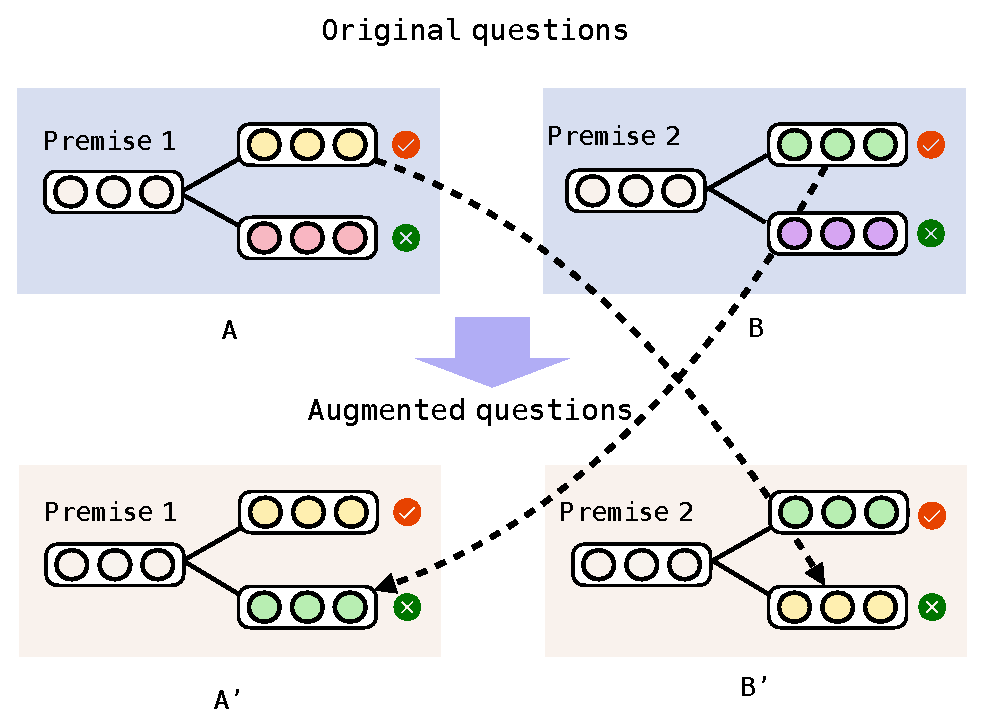
\includegraphics[width=\columnwidth]{figure/cross.eps}
\caption{The Crossover Operation: the true choice of both questions
are used to replace the false choices of these questions to create
two new proxy questions.}
\label{fig:cross}
\end{figure}

Compared to all other operations in classes 1 and 2, the crossover provides a proxy question that is most different from the original one but easier from a human perspective. This is because the two choices may be quite unrelated. If the model does not handle it correctly, it may be more indicative of a short circuit. As a result, the crossover is potentially a better short circuit test than others.

Another advantage of the crossover operation is that we can generate multiple false choices for an original question at a low cost, allowing us to test each original question more thoroughly. In contrast, most other operations cannot produce an adequate number of different variants of the original choice.

In summary, the proposed black-box choice operator provides a more generalizable and model-independent method for detecting short circuits in MCQ models. By applying various operations to create proxy questions, we can assess the model's performance and robustness more accurately, contributing to the development of better and more reliable models in the future.

\subsection{Improving Model Robustness by Data Augmentation}

If a model is shown to short-circuit by the proxy tests, its performance may decline, especially when applied to out-of-domain test data. To make models more robust, one natural thought is to generate more data to encourage models to focus on the relation between the premise and choices. While the operations used to generate proxy tests can also be utilized for data augmentation, not all of them are scalable or able to generate enough data for training.

The two operations that can generate a substantial amount of data are crossover and mutation. These operations can be applied to the training data to enhance the model's robustness.

\subsubsection*{Crossover for Data Augmentation}

Crossover is a good option for data augmentation because the two choices were originally true answers in their respective questions and presumably carry spurious features if the model was short-circuiting. By incorporating crossover into the training data, the model is forced to consider the premise in order to determine which choice is better.

\subsubsection*{Mutation for Data Augmentation}

Mutation has two flavors: (1) swap the words only in the true choice; (2) swap the words both in the true and the false choice. Compared to crossover, mutation has the potential to be more effective at improving model robustness. It not only forces the model to look into the premise due to its two very similar choices (same set of tokens), but also makes the model more sensitive to fine differences in word orders and enhances the model's prior grammatical knowledge.

\subsubsection*{Differentiating between Proxy Test and Data Augmentation}

It is essential to differentiate between the use of crossover and mutation operations in proxy tests and data augmentation. In proxy tests, these operations are used to modify the test data to assess the model's short-circuiting behavior. In contrast, when applied for data augmentation, the same operations work on the training data to enhance the model's robustness and generalization capabilities.

In conclusion, data augmentation through crossover and mutation operations can contribute to improving model robustness by encouraging models to focus on the relationship between the premise and choices. By incorporating these operations into the training data, models are forced to consider the premise and become more sensitive to the fine differences in word orders, leading to better performance and reliability in real-world applications.

\section{Experiments}
In this section, 
% after introducing the datasets we construct from multiple business lines, 
% we discuss our experimental results under single- \& multi-domain product categorization scenarios. A brief comparison of time efficiency between $\mathsf{TaLR}$ and simple \textit{Reranking} is also included. We also discuss the generalizability of $\mathsf{TaLR}$ under zero-shot conditions (evolving taxonomy  \& new taxonomy). 
we discuss experimental results under static multi-domain settings and dynamic (taxonomy evolving \& new taxonomy) conditions. A brief comparison of time efficiency between $\mathsf{TaLR}$ and simple \textit{Reranking} is also included.

% \subsection{Dataset Analysis}

\subsection{Baselines}
\label{sec: baseline}
% \TODO{Intro: TF-IDF+LR, fastText, BERT, multi-task,...}
We implement several baseline methods based on single-domain, multi-domain, and dynamic scenarios. 
To ensure fair comparisons, we also experiment concatenating product titles with meta concept text as input for some competitive baselines.
% \subsubsection{Single-domain}
% For methods targeting single-domain categorization tasks, we train individual models for each business. 
% As a system to be deployed in production environment with limited resources, 
Note that all the strong baselines are practicable in our online production environment, and those with unbearable space or time complexity are not considered. 
% We only choose practicable baselines that meet our production environment and 
Works holding different assumptions (e.g. necessitate multi-label or not support Chinese) with us are not considered either. 
Finally, we deploy and benchmark the following common baselines: 

\textit{Flat Classifier} \textbf{TF-IDF\&LR} represents product titles with TF-IDF weighted dense vectors, and executes classification with Logistic Regression. \textbf{FastText} \cite{bojanowski2017enriching} is a common baseline adopted in online product categorization challenges. 
% We also utilize pretrained 
\textbf{BERT} classifier is used as the strong baseline in both single-domain and multi-domain (trained with multi-task learning) settings.

\textit{Hierarchical Classifier} \textbf{HMCN}~\cite{wehrmann2018hierarchical} and \textbf{HiMatch}~\cite{chen2021hierarchy} leverage hierarchical information from taxonomy to 
guide the classification process, and we use BERT as a text encoder in both approaches. 
\textbf{XR-Linear} and \textbf{XR-Transformer} are two derivatives of PECOS~\cite{yu2020pecos} framework for extreme classification, which achieve competitive performance in most open product categorization datasets.

% HiMatch implicitly models hierarchical knowledge via GCN and positive \& negative node sampling.

% \subsubsection{Multi-domain}
% We exploit \textbf{multi-task} learning paradigm as strong baseline for multi-domain categorization. 
% % A shared BERT is utilized as the text encoder with multiple output heads targeting different tasks. 
% Data batches from each task take turns to update the model weights during training, and the loss function is formulated by summing up multi-class cross-entropy losses across different tasks.
% \subsubsection{Zero-shot Setting}
% \textit{Zero-shot Classifier} Since all the above baselines cannot tackle taxonomy evolving issues
% % (evolving taxonomy  \& new taxonomy) 
% without re-training, we adopt the vanilla BERT to encode both product titles and category names and calculate their [$\mathtt{CLS}$] similarity as a naive baseline \textbf{BERT-matching}. We further utilize separate BERT classifiers trained with few-shot data (1\%) on each task respectively as a strong baseline \textbf{BERT-few-shot}. \TODO{delete and move to each sub section}
% While each component of $\mathsf{TaLR}$ could be used individually under zero-shot scenarios, the ablations of $\mathsf{TaLR}$ can also be regarded as competitive zero-shot alternatives. 

\subsection{Experimental Setup}
We mix up training data from three datasets to train the unified $\mathsf{TaLR}$. 
We use \textbf{accuracy} score as the evaluation metric to meet real-world business demands.
Accuracy mathematically equals to \textbf{Micro-F1} score in a single-label multi-class classification problem. More details can be found in Appendix~\ref{appdix:exp detail}.

\subsection{Overall Results}
\label{sec:all res}

\begin{table}[!th]
\small
\setlength{\tabcolsep}{3.5pt}
  \begin{threeparttable}[b]
  \caption{The accuracy of baselines and our $\mathsf{TaLR}$ framework with variants on static multi-domain datasets. The best results are \textbf{bolded}, and the best baseline results are starred. Overall accuracy is the weighted average w.r.t respective test set size. $\mathsf{MS}$: mapping scorer, $\mathsf{CL}$: contrastive learning. 
  % ``+concept'' means concatenation of concepts after the product title, and (-) means ablation. 
  % \xiujie{(+) ... ablation?}
  }
  \label{tb:all}
  \centering
  \begin{tabular}{l|llll}
    \toprule
    Methods & Overall & \multicolumn{1}{c}{QD} & \multicolumn{1}{l}{\;BH} & \multicolumn{1}{l}{\;FG}\\
    \midrule
    \multicolumn{5}{c}{Separate models}\\
    \midrule
    TF-IDF\&LR $ $ & 69.51 & 69.93 & 68.23 & 69.95 \\
    FastText $ $ & 74.62 & 74.01 & 71.68 & 80.82 \\
    BERT $ $ & 83.49 & 84.82 & 79.93$^*$ & 84.23\\
    BERT+$\spadesuit$  $ $ & 83.01 & 86.45 & 79.02 & 75.32\\
    % HFGN-F-classifier $ $ & - & 83.72 & 77.09 & 84.25 \\
    HMCN-F-BERT $ $ & 82.14 & 83.72 & 77.09 & 84.25 \\
    HiMatch-BERT $ $ & 84.08 & 86.12 & 77.38 & 84.19 \\
    HiMatch-BERT+$\spadesuit$$ $ & 83.75 & 87.26$^*$ & 77.26 & 78.53 \\
    XR-Linear$ $ & 76.57& 75.27 & 77.91 & 78.95 \\
    XR-Transformer$ $ & 84.58$^*$ & 79.74 & 79.23 & 84.58$^*$ \\
    XR-Transformer+$\spadesuit$$ $ & 81.45 & 85.34 & 74.59 & 78.53  \\
    \midrule
    (a): $\mathsf{TaLR}$ $ $ & 85.90 & 87.88 & 81.92 & 85.09\\
    \midrule
    \multicolumn{5}{c}{Unified model}\\
    \midrule
    % BERT Multi-task & 64.41 & 76.79 & 50.26 & 44.09 \\
    BERT Multi-task & 68.00 & 80.27 & 50.28 & 44.29 \\
    BERT Multi-task+$\spadesuit$ & 67.79 & 81.37 & 49.77 & 39.83 \\
    (b): $\mathsf{TaLR}$ & \textbf{86.23} & \textbf{88.16} & \textbf{82.48} & \textbf{85.25}\\
    \midrule
    \multicolumn{5}{c}{$\mathsf{TaLR}$ ablation test}\\
    \midrule
    % (-) rerank stage & {82.29}  & 84.19  & {77.63}  & 82.72 \\
    % (-) retrieval stage & 83.29  & 84.95  & 80.53  & {81.78} \\
    % \midrule
    % \midrule
    (c): (b) (-) $\mathsf{CL}$ & 85.26  & 86.83  & 81.75  & 85.13 \\
    (d): (b) (-) $\mathsf{MS}$ & {84.63}  & {86.59}  & {80.13}  & {84.71}  \\
    (e): (b) (-) $\mathsf{CL}$\&$\mathsf{MS}$ & 82.82 & 83.85 & 79.15 & 84.71 \\
    (f): (b) (-) $\mathsf{CL}$\&$\mathsf{MS}$ +$\spadesuit$ & 84.38 & 87.43 & 80.64 & 79.77 \\

    % (-) vector-based retrieve & 84.91  & 86.52  & 81.66  & 84.28  \\

    \bottomrule
  \end{tabular}
  \begin{tablenotes}
    % \item[1] The overall accuracy is the weighted average of results on three domains, where weights are determined by the size of their corresponding test set.
    % We list separate accuracy on each subset.
    % \item[2] Methods with $ $ notation train three separate models on the three datasets of business lines and infer using its corresponding model. Methods without $ $ only train one unified model using multi-domain data.
    % \item[3] (-) denotes the ablation of following modules in $\mathsf{TaLR}$.
    \item[$\spadesuit$] concatenate concept text after product title
    \item[(-)] ablate cretain modules
    % \item[$\mathsf{MS}$] mapping scorer module
    % \item[$\mathsf{CL}$] contrastive learning module
  \end{tablenotes}
  \end{threeparttable}
\end{table}
The overall accuracy score is shown in \tabref{tb:all}.
% , and we can make the following observations.
Since traditional single-domain approaches cannot tackle \textbf{multi-domain taxonomies}, we train \textbf{separate} models on each business respectively. 
Among methods targeting one static taxonomy, hierarchical classifiers generally perform better than flat classifiers
% mainly because it leverages 
with the aid of taxonomy structure information.
% utilizes the positive and negative relationship of nodes in taxonomy.
However, because these methods can only handle one static taxonomy, they not only suffer from efforts to maintain different models for each domain but also fail to leverage multi-domain data. 
While the multi-task BERT is able to train and infer on three domains within one model, it performs even worse than TF-IDF\&LR on BH and FG. 
One possible reason is that the multi-task approach relies heavily on the weighting of losses, and if the task-specific training data distribution varies significantly, one task might dominate the joint distribution and constrain the optimization of other tasks. 
% Straightforwardly 
Simply concatenating meta concepts to titles does not always take effect,
% for these methods on some domains, 
and this is expected since concatenated tokens implicitly contribute to the joint representation of one sentence (e.g. self-attention in transformer), which proves to be inferior to our explicit usage of statistical mapping and contrastive grouping.
% this is expected since short concept texts can not dominate the surface form of titles, and these methods does not optimize relatedness in a macroscopic view. \zelin{not clear}


For our proposed framework $\mathsf{TaLR}$, variant (a) already outperforms other baselines in separate model training paradigm, while $\mathsf{TaLR}$ (b) further achieves even higher accuracy when jointly trained on the mixed multi-domain data where the multi-task BERT fails,
verifying $\mathsf{TaLR}$'s efficacy on \textbf{multi-domain taxonomies}. 
% As is shown, the unified $\mathsf{TaLR}$ (b) is better than separate $\mathsf{TaLR}$ (a), and 
We assume that the measurement of semantic relatedness is transferable on either business domain, and their shared knowledge could be integrated via contrastive pretraining as well. 
% We assume that some products and category names from multiple domains 
% may share similar semantic meanings as well as concepts knowledge, 
Therefore, the unified training helps improving the performance on each respective domain instead of conflicting each other as BERT multi-task does. 
% This is our cross-domain \textbf{knowledge integration} assumption and is thus verified. 
% \zelin{not clear}
% \zelin{not perspicuous}
% Furthermore, when we compare $\mathsf{TaLR}$ (-) reranking (a single BERT bi-encoder) and $\mathsf{TaLR}$ (-) retrieval (a single BERT cross-encoder) with the BERT-classifier, the results is close. 
% This first elucidates that these two stages are reinforcing each other, and further corroborates that the improvement of $\mathsf{TaLR}$ from $\mathsf{TaLR}$ $ $ is contributed by the \textbf{knowledge integration} capability of the framework instead of purely addition of data.

From the ablation tests, we can observe the effectiveness of the two plug-in modules in our $\mathsf{TaLR}$ framework from row (c) and (d), and the contribution of these two modules are orthogonal. 
Removing the mapping scorer in (d) drops the overall accuracy most, 
while removing contrastive pretraining in (c) results in its inferior performance than (a) as well. 
This indicates both modules are indispensable for the enhancement of exploiting multi-domain data.
% Compared with (e)$\rightarrow$(c) and (e)$\rightarrow$(d), (e)$\rightarrow$(f) improves the least in overall accuracy, showing that our two plug-in modules are more effective than simply concatenation of concepts. 
From (e)$\rightarrow$(f), concatenating meta concepts somehow improves the overall performance, but (f) still loses to (b). This reaffirms our above assumption that our usage of meta concepts is superior to simple concatenation. 
% \zelin{no key point}
% showing that our model with concept grouping can semantically align the embeddings of product titles and category names from multiple domains. 
% Removing the concept retrieval unit impairs the overall results significantly, mainly on account of the external knowledge imported from the concept set. 
To further analyze the effects of the two plug-in modules, we conduct Case Study in Appendix~\ref{sec:appdix-case}.

\subsection{Time Consumption} 
\label{sec:time cons}
% A big concern of our framework is to limit the run-time overheads, since the large label space challenge may deteriorate in one-vs-all retrieval systems rather than classification approaches.  
To meet online deployment requirement, the inference time consumption (seconds cost for each instance) needs to be considered. We compare $\mathsf{TaLR}$ with the vanilla model (single BERT cross-encoder) on the three datasets in \figref{fig:time}.
% , and we train and test on our three standard datasets. 
% Here the single BERT cross-encoder computes the similarity score over all category classes and selects the most similar one as the prediction, while $\mathsf{TaLR}$ instead utilized bi-encoder with cached category embeddings to conduct one-vs-all retrieval and the cross-encoder BERT in \textit{Reranking} stage takes only 10 candidates. 
% \figref{fig:time} plots the relationship between the number of classes and the inference time. 
On the one hand, the inference speed of $\mathsf{TaLR}$ is much faster (4 times faster for FG and 10 times faster for BH) than vanilla model owing to the \textit{Retrieval} stage. On the other hand, the time consumption per item of $\mathsf{TaLR}$ increases almost linearly along with the number of classes, while for vanilla model the overhead grows more sharply, revealing the time efficiency of $\mathsf{TaLR}$ when the class number scales up. 
% As for the accuracy score, $\mathsf{TaLR}$ fluctuates in the same pace with BERT cross-encoder but consistently outperforms it, and the reason of fluctuation is explained before.
% $\mathsf{TaLR}$ also consistently outperforms single BERT cross-encoder in accuracy due to the selection of better candidates in \textit{Retrieval} stage. 

\begin{figure}[thbp] \centering
    \includegraphics[width=0.4\textwidth]{time.pdf}
    \caption{Accuracy results and inference time consumption when the number of classes grows.} 
    \label{fig:time}
\end{figure}

\subsection{Dynamic Test Set Experiment}
\label{sec:evolve res}
In order to evaluate the ability of our framework on \textbf{taxonomy evolving} challenge, 
we use $\mathsf{TaLR}$ trained on the original multi-domain datasets to directly infer on two dynamic test sets. The vanilla BERT without any finetuning is a naive baseline \textbf{BERT-matching}. The BERT fine-tuned with few-shot new data (1\%) is a strong baseline \textbf{BERT-few-shot}.
% we directly infer product titles with $\mathsf{TaLR}$ trained on multi-domain datasets on the evolved taxonomies.
% we conduct experiments to directly infer evolved new category of the product with $\mathsf{TaLR}$. 
Here ``before'' denotes the subset from the original test set and ``after'' denotes the subset with the same product titles but evolved categories.
From the listed accuracy ``before'' and ``after'' taxonomy evolving in \tabref{tb:evolve}, we can conclude that $\mathsf{TaLR}$ sustains satisfactory accuracy compared with its strong counterpart trained with 1\% extra data.
% the encoded [$\mathtt{CLS}$] token similarity from %%% explained before
% BERT-matching is the vanilla similarity matching baseline and BERT-few-shot is the separate few-shot classifiers we mentioned in \secref{sec: baseline}. Note that BERT-few-shot is trained on full data before evolving.

\begin{table}[th]
\small
\setlength{\tabcolsep}{1.8pt}
  \begin{threeparttable}[b]
  \caption{The accuracy on two dynamic test sets. $\Delta$ is the change
  of accuracy after evolving. The best ``after'' scores and least drop $\Delta$ are bolded.}
  \label{tb:evolve}
  \centering
  \begin{tabular}{l|ccc|ccc}
    \toprule
    \multirow{2}{*}{Methods} & \multicolumn{3}{c|}{QD$-divide$} & \multicolumn{3}{c}{QD$-integrate$}\\
    \cline{2-7}
    & Before & After & $\Delta$ & Before & After & $\Delta$ \\
    \midrule
    BERT-matching & 6.66 & 11.95 & \textbf{+5.29} & 13.39 & 2.23 & -11.16\\
    BERT-few-shot & 90.51 & 43.54 & -46.96 & 86.79 & 50.16 & -36.53\\
    \midrule
    $\mathsf{TaLR}$ & 90.11 & \textbf{69.71} & -20.40 & 85.20 & \textbf{81.48} & \textbf{-3.72}\\
    % (-) contrastive  & 89.10 & \textbf{79.21} & -9.89 & 84.11 & 80.02 & -4.09\\
    % (-) rerank stage & 89.70 & 73.94 & -15.76 & 86.36 & 81.47 & -4.89\\
    % (-) rule-based unit & 89.51 & 64.25 & -25.26 & 84.61 & 81.19 & \textbf{-3.42}\\
    \bottomrule
  \end{tabular}
%   \begin{tablenotes}
%     \item[1] 
%   \end{tablenotes}
  \end{threeparttable}
\end{table}
% {too long, rewrite}
% On the one hand, our $\mathsf{TaLR}$ even outperforms BERT-few-shot without additional training on evolved taxonomies, which indicates its robustness in handling dynamic issues.
% On the other hand, we can observe an opposite trend of BERT-matching and $\mathsf{TaLR}$ through $\Delta$ when two different evolving challenges are encountered. In the node $integrate$ scenarios, $\mathsf{TaLR}$ exhibits robustness with a slight drop of accuracy. 
% When progressively ablating contrastive learning and the whole \textit{Reranking} stage, the accuracy of $\mathsf{TaLR}$ consistently decreases, which indicates their contributions to the node \textit{integrate} variants in evolving taxonomy.
% % \textbf{Taxonomy integration}.
% % On the other hand, BERT-matching suffers from a drastic drop in accuracy, which may attribute to 
% However in the node $divide$ scenario, wherever contrastive learning is incorporated, there is a substantial drop in $\Delta$. Completely excluding the contrastive learning while keeping all other components gives the best accuracy. 
% The reason behind it is that contrastive learning tends to make the representations of products from the same category tied closer, while the division of nodes breaks this relation. 


\subsection{Extrapolating Results on New Taxonomy}
\label{sec:new tax}

% For multi-domain business lines, 
Consider an extreme \textbf{taxonomy evolving} condition when a new business line emerges, a robust model is supposed to categorize incoming products based on the brand-new taxonomy. 
% Hence it poses challenge for $\mathsf{TaLR}$ to zero-shot transfer to new domains so as to improve user experience in this cold-start scenario.

\begin{table}[th]
%   \begin{threeparttable}[b]
  \small
  \caption{The accuracy of $\mathsf{TaLR}$ on the new taxonomy. }
  \label{tb:zeroshot}
  \centering
  \begin{tabular}{l|ccc}
    \toprule
    Methods & QD & BH & FG \\
    \midrule
    BERT-matching & 9.00 & 11.23 & 4.03 \\
    BERT-few-shot & 43.29 & 35.19 & 29.80 \\
    % BERT-product & 52.00 & 48.81 & 51.32 \\
    \midrule
    $\mathsf{TaLR}$ & \textbf{60.57} & \textbf{65.45} & \textbf{62.69}\\
    % $\mathsf{TaLR}$-few(?) &  &  & \\
    % $\mathsf{TaLR}$-finetune(?) & 84.32 & 76.40 & 83.59\\
    % \midrule
    (-) contrastive & 56.71 & 64.99 & 60.79\\
    % (-) Rerank stage & 53.79 & 59.56 & 57.68 \\
    (-) mapping scorer & 56.25 & 64.65 & 59.29\\
    \bottomrule
  \end{tabular}
%   \begin{tablenotes}
%     \item[1] 
%   \end{tablenotes}
%   \end{threeparttable}
\end{table}

We deploy our experiments in a zero-shot manner, where we take turns to train $\mathsf{TaLR}$ on either two business data and test its performance on the remaining business. $\mathsf{TaLR}$ still outperforms BERT-few-shot. 
% We compare $TaLR$ with BERT-matching model and bi-encoder BERT in zero-shot, and $TaLR$-zero sustains better accuracy, 
% This indicates that $\mathsf{TaLR}$'s ability capturing semantic relatedness between product titles and category names on original domains could be seamlessly transferred to new domains with new taxonomies.
This shows $\mathsf{TaLR}$'s preeminent transferability with the reformulation of textual semantic matching, which helps improving user experience in this cold-start scenario.
% It mainly contributes to the learning in the other two domains, 
% which enhances the semantic relatedness understanding in the third dataset with brand new taxonomy.
Each component in the ablation test verifies its effectiveness as well. 

% More details about ablation setting is in \secref{sec:exp detail}.



% \subsection{Different Retrieval Strategies}
% \label{sec:retri stra}
% In \textit{Retrieval} stage, it is encouraged to exploit the potential candidates as accurately as possible, otherwise the latter \textit{Reranking} stage would never make right predictions if the true label is not covered by the retrieved candidates. Hence we use HR@$k$ to measure the retrieval performance.

% Firstly, we compare several alternatives of the loss function in vector-based retrieval model. In \figref{fig:vector-retri}, as $k$ goes on, the HR score increases, and the model trained with Cosent loss is consistently better than others, while the model trained with SBERT loss performs unstably, sometimes worse than Cosine loss. 
% One explanation is that comparing with Cosine loss and SBERT loss, the Cosent loss focuses on the positive-versus-negative pairwise optimization, which means the model only cares for the relative order of the prediction results instead of the specific value. And this setting brings consistent recall of candidates.
% \begin{table}[th]
%   \caption{The retrieval results of the vector-based unit over different loss function. The best results are bolded.}
%   \label{tb:vector-retrieval}
%   \centering
%   \begin{tabular}{c|c|ccc}
%     \toprule
%     Loss & Dataset & HR@1 & HR@5 & HR@10 \\
%     \midrule
%     \multirow{3}{*}{Cosine} & QD & 74.80 & 82.28 & 84.46\\
%     & BH & 72.75 & 81.77& 84.04\\
%     & FG & 65.59 & 80.40 & 83.23\\
%     \midrule
%     \multirow{3}{*}{SBERT} & QD & 82.25 & 88.96 & 90.92\\
%     & BH & 76.95 & 86.76 & 89.41\\
%     & FG & 80.67 & 87.27 & 88.86\\
%     \midrule
%     \multirow{3}{*}{Cosent} & QD & 84.19 & 88.97 & 90.30\\
%     & BH & 77.64 & 85.27 & 87.18\\
%     & FG & 82.72 & 86.66 & 87.48\\
%     \bottomrule
%   \end{tabular}
% \end{table}

% \begin{figure}
%   \begin{subfigure}[b]{0.49\columnwidth}
%   \centering
%   \includegraphics[width=\columnwidth]{hr_1.pdf}
%   \caption{HR@1}
%   \end{subfigure}
% %   \hfill
% %   \begin{subfigure}[b]{0.49\columnwidth}
% %   \centering
% %   \includegraphics[width=\columnwidth]{hr_5.pdf}
% %   \caption{HR@5}
% %   \end{subfigure}
%   \hfill
%   \begin{subfigure}[b]{0.49\columnwidth}
%   \centering
%   \includegraphics[width=\columnwidth]{hr_10.pdf}
%   \caption{HR@10}
%   \end{subfigure}
%   \caption{The retrieval results of the vector-based unit over different loss functions.}
%   \label{fig:vector-retri}
% \end{figure}

\cut{
To generate better candidates, we adopt several heuristic algorithms for two-way candidates fusion.
% the vector-based unit and rule-based unit. 
\tabref{tb:fusion} depicts the retrieval results over different fusion strategies. The size of merged candidate sets is not stuck to $10$ for some of the strategies, so we list the average number.
Generally, the \textbf{Rule-First} algorithm achieves better scores, and \textbf{De-Dupli} algorithm is competitive with it. We use \textbf{Rule-First} in our framework due to its fixed candidate size which is more convenient to process.
Although the pure vector-based unit performs less effectively than the rule-based counterpart, they could complement each other after fusing together with the help of an ensembled understanding of textual semantics and training set distribution.
% the ensemble of vector-based unit and rule-based unit strengthens the performance of rule-based unit, revealing that vector-based unit can better understand the instance semantically that rule-base unit can not. 
More discussions are in Case Study.

\begin{table}[th]
\setlength{\tabcolsep}{2pt}
  \caption{The retrieval results of candidates for different fusion strategies. The best results are bolded.}
  \label{tb:fusion}
  \centering
  \begin{tabular}{c|cc|cc|cc}
    \toprule
    \multirow{2}{*}{Strategy}  & \multicolumn{2}{c|}{QD} & \multicolumn{2}{c|}{BH} & \multicolumn{2}{c}{FG} \\
    \cline{2-7} 
      & Recall & Size & Recall & Size & Recall & Size \\
    \midrule
    Rule-based & 95.33 & 8.6 & 96.77 & 8.8 & 97.32 & 9.0 \\
    Vec-based & 90.30 & 10 & 87.18 & 10 & 87.48 & 10 \\
    \midrule
    De-Dupli & 96.08 & 10.5 & \textbf{97.54} & 10.4 & 97.77 & 10.7 \\
    Norm\&Rank & 93.74 & 10 & 92.42 & 10 & 92.77 & 10 \\
    Rule-First & \textbf{96.12} & 10 & 97.48 & 10 & \textbf{98.01} & 10 \\
    \bottomrule
  \end{tabular}
\end{table}
}
% \section{Case Study}
% For product ``\textit{red dancing shoes (size 35)}'', which should be categorized to \verb|Sports/Outdoors| $\rightarrow$ \verb|Yoga/Dancing| $\rightarrow$ \verb|Dancing Shoes|, the vector-based unit retrieves the correct class as top-$1$ answer, but the rule-base unit retrieves \verb|Clothes/Shoes| $\rightarrow$ \verb|Woman Shoes| $\rightarrow$ \verb|Woman Slippers| as top-$1$. This time the distribution knowledge guides the rule-based model towards a wrong direction, while the vector-based model succeeds relying on the semantic similarity.

% For product ``\textit{CHEERS$^\circledR$ 12 years}'', the vector-based model categorizes it to \verb|Books| $\rightarrow$ \verb|Economics/Management| $\rightarrow$ \verb|Marketing|, whereas the rule-based unit correctly retrieves \verb|Alcoholic Drinks| $\rightarrow$ \verb|Imported Liquors| $\rightarrow$ \verb|Whisky|. This shows that ``12 years'' misleads the vector-based model to the semantic meaning of economics, and rule-based unit successfully leverages its distribution knowledge in training set.

% For product ``\textit{towel gourd\&soy bean (towel gourd 1 pcs, soy bean 150g)}'', both rule-based unit and vector-based unit predict
% \verb|Vegetable| $\rightarrow$ \verb|Soy Product| $\rightarrow$ \verb|Soy Bean| wrongly as top-$1$, whereas $\mathsf{TaLR}$ classifies it to correct \verb|Vegetable| $\rightarrow$ \verb|Mixed Product| $\rightarrow$ \texttt{Vegetables mixture}, and clearly, the contribution is from the following \textit{Reranking} stage.
% \begin{table*}[t]
%   \caption{The retrieval results of candidates for different fusion strategies. The best results are bolded.}
%   \label{tb:fusion}
%   \centering
%   \begin{tabular}{c|c}
%     \toprule
%     Product title & \textit{red dancing shoes (size 35)} \\
%     \midrule
%     Ground truth & \verb|Sports/Outdoors| $\rightarrow$ \verb|Yoga/Dancing| $\rightarrow$ \verb|Dancing Shoes| \\
%     Vector-based top-$1$ & \verb|Sports/Outdoors| $\rightarrow$ \verb|Yoga/Dancing| $\rightarrow$ \verb|Dancing Shoes| \\
%     Rule-based top-$1$ & \verb|Clothes/Shoes| $\rightarrow$ \verb|Woman Shoes| $\rightarrow$ \verb|Woman Slippers| \\
%     \midrule
%     Product title & \textit{CHEERS$^\circledR$ 12 years} \\
%     \midrule
%     Ground truth & \verb|Alcoholic Drinks| $\rightarrow$ \verb|Imported Liquors| $\rightarrow$ \verb|Whisky| \\
%     Vector-based top-$1$ & \verb|Books| $\rightarrow$ \verb|Economics/Management| $\rightarrow$ \verb|Marketing| \\
%     Rule-based top-$1$ & \verb|Alcoholic Drinks| $\rightarrow$ \verb|Imported Liquors| $\rightarrow$ \verb|Whisky| \\
%     \midrule
%     Product title & \textit{towel gourd \& soy bean (towel gourd 1 pcs, soy bean ~150g)} \\
%     \midrule
%     Ground truth & \verb|Vegetable&/ Product| $\rightarrow$ \verb|Mixed Product| $\rightarrow$ \verb|Vegetables mixture| \\
%     Vector-based top-$1$ & \verb|Vegetable/&Soy Product| $\rightarrow$ \verb|Soy Product| $\rightarrow$ \verb|Soy Bean| \\
%     Rule-based top-$1$ & \verb|Vegetable/Soy Product| $\rightarrow$ \verb|Soy Product| $\rightarrow$ \verb|Soy Bean| \\
%     \bottomrule
%   \end{tabular}
% \end{table*}



\subsection{Online Experiment}
% We conduct online experiments on one downstream task where the category of a product is needed, 
% % of semantic vector space, 
% that is the main page recommendation (multi-domain). 
% % After deploying our contrastive pretrained model to compute the hidden vector representations of related products and utilizing this in sophisticated 
% When $\mathsf{TaLR}$ is incorporated in the
% recommendation system, customer purchase click rate increases significantly over 5\%.
We conduct online experiments on one downstream task where $\mathsf{TaLR}$'s domain-independent category recognition ability helps transfer user preferences from other domains and contributes to a more accurate recommendation. When $\mathsf{TaLR}$ is incorporated in the recommendation system, customer seasonal purchase revenue increases significantly over 5\%.
\section{Related Work}
This section surveys previous works on question generation and tree encoding
respectively.

Text question generation has attracted the attention 
after the work of ~\citeauthor{du2017learning}~\shortcite{du2017learning}, who uses deep seq2seq model 
to generate questions from a raw text paragraph. 
Before that, text question generation relied heavily on hand-craft 
question patterns~\cite{HeilmanS10,LabutovBV15,MostowC09} which is time and 
labor consuming. 

However, this pure seq2seq model is not focused and 
has no control over part in the paragraph to generate question. 
~\citeauthor{zhou2017neural}~\shortcite{zhou2017neural} proposed to encode 
key phrase information using binary indicators to generate 
key-aware questions and they assumes the answer to be key phrase. 
Considering key phrase (answer) is unavailable in reality, 
~\citeauthor{SubramanianWYT17}~\shortcite{SubramanianWYT17} applied 
a two-stage approach. First, key phrases are extracted by 
pointer network~\cite{ptrnet}. Second, 
key phrases are encoded in the same way as 
Zhou et al. With the intuition that questions could be asked in many ways, 
~\citeauthor{Yao2018vae}~\shortcite{Yao2018vae} used conditional-VAE to 
increase the diversity of questions. More recently, models with 
auxiliary feature information~\cite{HarrisonW18} helped improve 
the question quality. Structure question generation aims at 
converting structured data such as triples in knowledge graph to questions. 
~\citeauthor{SerbanGGACCB16}~\shortcite{SerbanGGACCB16} proposed a model to generate factoid questions from knowledge base triples.  None of the above work
considered using parse tree structures to aid question generation process,
which is the focus of this paper.

Sequential RNN model takes sentence as a sequence of words, 
ignoring the syntactic information. In order to utilize
such syntactic information with sequential information, 
~\citeauthor{tai2015improved}~\shortcite{tai2015improved} proposed Tree-LSTM to 
encode the binary parse tree recursively in a bottom-up fashion to 
classify sentiment. In text generation task, 
\citeauthor{eriguchi2016tree}~\shortcite{eriguchi2016tree} 
proposed a tree-to-sequence model with attention mechanism to do 
machine translation and 
~\citeauthor{liang2018automatic}~\shortcite{liang2018automatic} proposed a 
tree-to-sequence model which could handle arbitrary trees, 
to do code comment generation. Our work is inspired by these previous
attempts and we are first to adapt structure encoded neural models to
textual question generations.
\section{Conclusion}
We implement a novel sequence-based dependency parsing
framework which takes advantage of high order features 
in parsing history. 
%We can also adapt beam search to this framework so as to
%relax the strictly greedy nature. Vine pruning\cite{rush2012vine} could
%be incorporated to speed up the parsing.
More importantly, we discovered that the parsing accuracy is very sensitive to
the quality of parsing sequence. Future work can be focused on
developing better sequence predictors that outperform Malt action classifier.
Furthermore, we use two sets of features for sequence predictor and
head mapper right now. A unified set of features between these two components
are worth exploring.
%Besides, better sequence predicting method and unified feature
%representation of two components are worth exploring.
%
%Though we currently get a not bad result,
%the sequence predictor still needs more exploration.
%According to our experiment, slightly changes
%on the sequence can lead to a fatal decline on accuracy. Ensuring the match degree of training sequence and testing
%sequence demands a high quality of sequence predictor.
%
%Further, the features in our current implementation are not expanded and well tuned yet  and we are free to define high order features to make use of parsing history. Our framework is flexible to merge other technics to enhance the performance. Introducing beam could make up for our greedy decoder and improve our accuracy. Vine pruning\cite{rush2012vine} could speed up parsing process. Besides, better sequence predicting method and unified feature representation of two components are worth exploring.


% Use \bibliography{yourbibfile} instead or the References section will not appear in your paper
% \nobibliography{aaai22}
\bibliography{sample-base}

% \section{Acknowledgments}

\end{document}
